\section{ساختار یک کامپایلر}
\begin{frame}{ساختار کلی}
\begin{itemize}\itemr
\item[-]
تا کنون به کامپایلر به عنوان یک جعبه دارای ورودی خروجی نگاه می‌کردیم،
\item[-]
اما اگر این جعبه را باز کنیم، با دو قسمت اصلی در کامپایلر‌ها مواجه می‌شویم:
\begin{enumerate}\itemr
\item 
آنالیز
\item 
سنتز
\end{enumerate}
\end{itemize}
\end{frame}

\begin{frame}{آنالیز}
\begin{itemize}\itemr
\item[-]
این قسمت، \lr{source code} را به قسمت‌های مختلفی می‌شکند،

\item[-]
و قواعد گرامی را به قسمت‌های مختلف تحمیل می‌کند.

\item[-]
این قسمت، اگر قسمتی را مخالف قوانین و گرامر زبان پیدا کند، پیام‌های مطلع کننده‌ای به کار نشان می‌دهد که ورودی را اصلاح کند.

\item[-]
و در پایان این قسمت، داده ساختاری به نام \lr{\textit{symbol table}} را تولید می‌کند که تقریبا در تمامی گام‌های کامپایل (که در ادامه به آنها پرداخته می‌شود،) استفاده می‌شود.
\end{itemize}
\end{frame}

\begin{frame}{سنتز}
\begin{itemize}\itemr
\item[-]
قسمت سنتز، بعد از رد شدن از تمامی مراحل قسمت آنالیز، خروجی مورد نیاز ما را تولید می‌کند.

\item[-]
به قسمت آنالیز 
\lr{front-end}
و قسمت سنتز
\lr{back-end}
هم گفته می‌شود.
\end{itemize}
\end{frame}

\begin{frame}{\lr{front-end}}
\begin{figure}[H]
\begin{center}
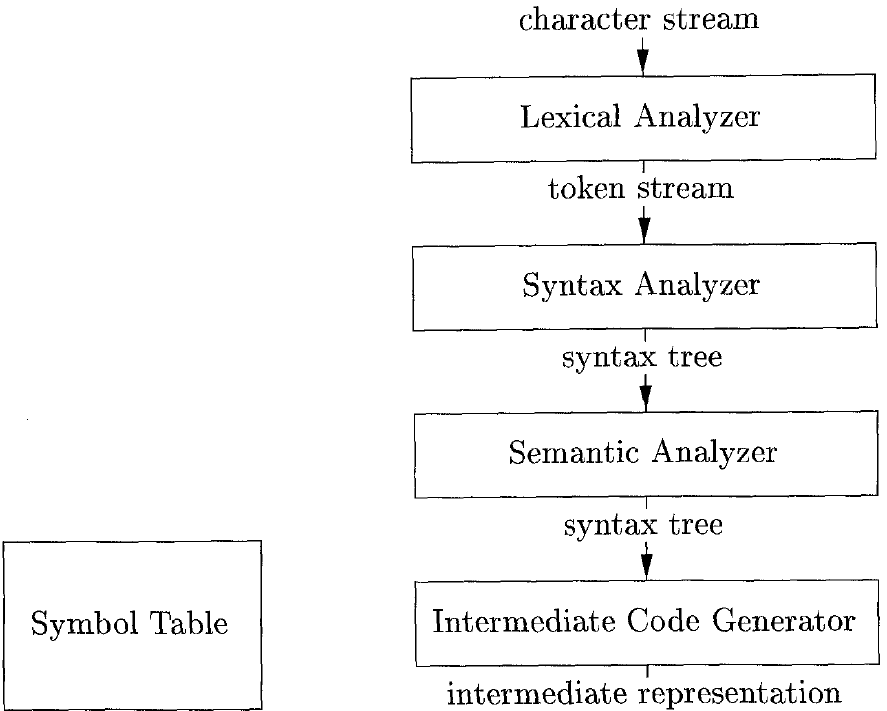
\includegraphics[width=0.5\textwidth, height=0.8\textheight, angle=-0.5]{docs/images/front}
\end{center}
\end{figure}
\end{frame}

\begin{frame}{\lr{back-end}}
\begin{figure}[H]
\begin{center}
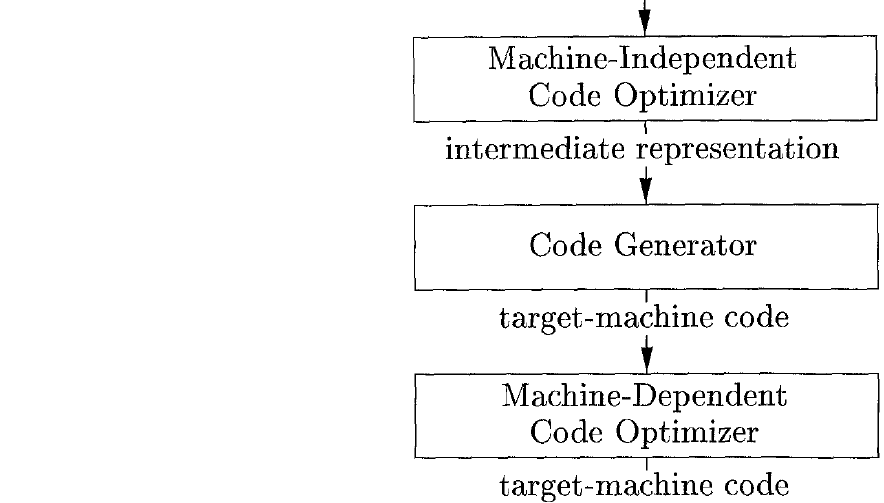
\includegraphics[width=0.5\textwidth, height=0.6\textheight, angle=-0.5]{docs/images/back}
\end{center}
\end{figure}
\end{frame}

\begin{frame}{تحلیل واژگانی \lr{(Lexical Analysis)}}
\begin{itemize}\itemr
\item[-]
اولین کار کامپایلر اسکن کردن فایل داده شده و شکستن آن به توکن‌های کوچک‌تریست که در آن زبان تعریف شده.

\item[-]
چیزی که تحلیل‌گر واژگان تولید می‌کند، دنباله‌ای از چنین ترکیبی‌ست:
\begin{equation*}
\left\langle\text{\lr{token-name}}, \text{\lr{attribute-value}}\right\rangle 
\end{equation*}
\end{itemize}
\end{frame}

\begin{frame}{تحلیل واژگانی \lr{(Lexical Analysis)}}
\begin{itemize}\itemr
\item[-]
فرض کنید چنین عبارتی را می‌خواهیم آنالیز کنیم:

\begin{flushleft}
\lr{\texttt{position = initial + rate * 60}}
\end{flushleft}
\item[-]
چیزی که تحلیل‌گر واژگان تولید می‌کند:
\begin{equation*}
\token{1} 
\left\langle\text{\lr{\texttt{=}}}\right\rangle
\token{2}
\left\langle\text{\lr{\texttt{+}}}\right\rangle
\token{3}
\left\langle\ast\right\rangle
\left\langle\text{\lr{\texttt{60}}}\right\rangle
\end{equation*}

\item[-]
که 
\lr{\textbf{id}}
مخفف 
\lr{identifier}
و عدد روبه‌روی آن اندیس 
\lr{symbol table}
است.
\begin{figure}[H]
\begin{center}
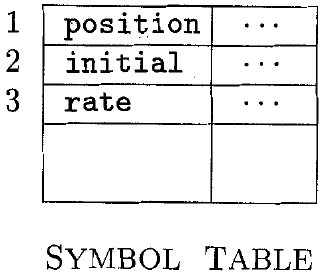
\includegraphics[width=0.25\textwidth, height=0.3\textheight]{docs/images/symboltable}
\end{center}
\end{figure}
\end{itemize}
\end{frame}

\begin{frame}{تحلیل نحوی \lr{(Syntax Analysis)}}
\begin{itemize}\itemr
\item[-]
سپس توکن به قسمت بعدی که تحلیل‌گر نحوی است فرستاده می‌شوند.

\item[-]
در این قسمت با توجه به گرامر زبان، یک ساختار درختی از توکن‌ها تولید می‌شود که با قواعد زبان سازگار است (یکی از قواعد تقدم عملگرهای ریاضیست)

\begin{figure}[H]
\begin{center}
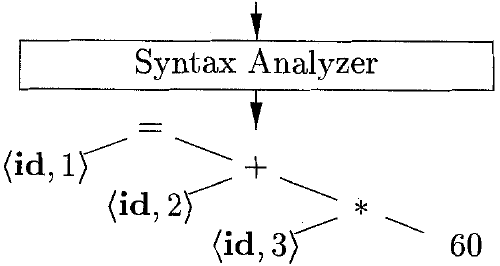
\includegraphics[width=0.25\textwidth, height=0.31\textheight]{docs/images/syntax}
\end{center}
\end{figure}
\end{itemize}
\end{frame}

\begin{frame}{تحلیل معنایی \lr{(Semantic Analysis)}}
\begin{itemize}\itemr
\item[-]
درخت تولید شده در مرحله‌ی قبل، به این قسمت فرستاده می‌شود.

\item[-]
در این قسمت، درخت تولید شده با اطلاعاتی دیگری همچون 
\lr{type}
متغیر‌ها بررسی می‌شود، و اگر تداخلی با زبان داشت، گزارش می‌شود. برای مثال یک زبان اجازه جمع شدن یک 
\lr{\texttt{float}}
با یک
\lr{\texttt{int}}
را نمی‌دهد که در این مرحله این اشتباه کشف و گزارش می‌شود.

\item[-]
همینطور، این قسمت اگر بتواند
\lr{type case}
مناسبی را انجام دهد، این کار را می‌کند. در مثال ما، متغیر‌های 
\lr{\texttt{position}}،
\lr{\texttt{initial}}
و 
\lr{\texttt{rate}}
از نوع
\lr{\texttt{float}}
تعریف شده‌اند و عدد 
\lr{\texttt{60}}
هم باید به 

\lr{\texttt{float}}
تبدیل می‌شود.

\begin{figure}[H]
\begin{center}
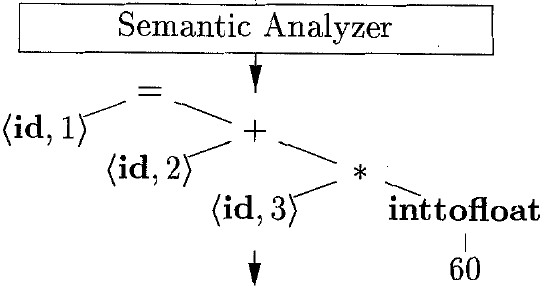
\includegraphics[width=0.3\textwidth, height=0.31\textheight]{docs/images/semantic}
\end{center}
\end{figure}
\end{itemize}
\end{frame}


\begin{frame}{تولید کد میانی \lr{(Intermediate Code Generation)}}
\begin{itemize}\itemr
\item[-]
کامپایلر‌های غالبا بعد از طی کردن مراحل قبل، کدی که بتوان آنرا بسادگی تولید و بسادگی ترجمه کرد را تولید می‌کنند تا سپس بتوانند آن را در مرحله‌ی بعدی بهینه کنند.
\vspace{5mm}
\begin{figure}[H]
\begin{center}
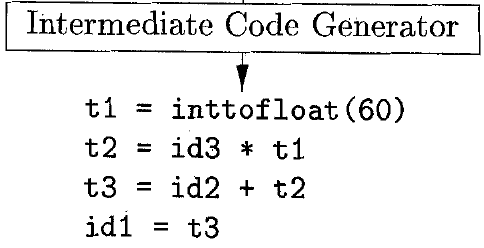
\includegraphics[width=0.3\textwidth, height=0.4\textheight, angle=1]{docs/images/intermediate}
\end{center}
\end{figure}
\end{itemize}
\end{frame}

\begin{frame}{بهینه‌سازی کد \lr{(Code Optimization)}}
\begin{itemize}\itemr
\item[-]
یکی از قسمت‌های بسیار مهم در کامپایلر‌های قسمت بهینه‌سازی کد است. کامپایلر‌های کنونی بسیار باهوش هستند و می‌توانند روند کدی که نوشته شده را بررسی با توجه به 
\lr{ISA}
معماری‌ای که برای آن می‌خواهند کد ماشین تولید کنند، بهترین دستورات را انتخاب کنند تا برنامه سریع‌تر اجرا شود.

\item[-]
به نظر شما یک کد اسمبلی که یک برنامه‌نویس آن را نوشته سریع‌تر است یا یک کدی که به زبان 
\lr{C}
نوشته شده و توسط یک کامپایلر مثل 
\lr{GCC}
یا 
\lr{Clang}
به اسمبلی ترجمه شده؟
\vspace{6mm}
\begin{figure}[H]
\begin{center}
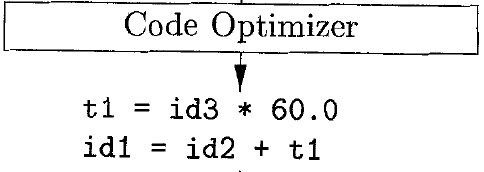
\includegraphics[width=0.25\textwidth, height=0.31\textheight, angle=1]{docs/images/optimizer}
\end{center}
\end{figure}
\end{itemize}
\end{frame}
